\begin{frame}{The Binomial Distribution}
    The \textbf{binomial distribution} is used to describe the number of successes in a fixed number of trials.
    \begin{itemize}
        \item This is an extension of the Bernoulli distribution.
        \item We check for a success or failure repeatedly over multiple trials.
        \item Each \textit{individual} trial can be described with a Bernoulli distribution.
    \end{itemize}
\end{frame}

\begin{frame}{Example: Insurance}
    \begin{itemize}
        \item Let’s return to the insurance agency where 70\% of individuals do not exceed their deductible.
        \item Suppose the insurance agency is considering a random sample of four individuals they insure. 
        \item What is the probability that exactly one of them will exceed the deductible and the other three will not? 
    \end{itemize}
\end{frame}

\begin{frame}{Example}
    Let’s call the four people Ariana ($A$), Brittany ($B$), Carlton ($C$), and Damian (D). Consider a scenario where one person exceeds the deductible:
\begin{align*}
    P&(A=\texttt{exceed}, B=\texttt{not}, C=\texttt{not}, D=\texttt{not}) \\
    &= P (A = \texttt{exceed})\times P (B = \texttt{not})\times P (C = \texttt{not})\times P (D = \texttt{not}) \\ 
    &= (0.3)\times(0.7)\times(0.7)\times(0.7) \\
    &= (0.3)^1\times(0.7)^3 \\
    &= 0.103
\end{align*}
\end{frame}

\begin{frame}{Example}
    \begin{itemize}
        \item But there are three other scenarios! 
            \begin{enumerate}
                \item Brittany could have been the one to exceed the deductible.
                \item ... or Carlton could have.
                \item ... or Damian.
            \end{enumerate}
        \item In each of these cases, the probability is $(0.7)^3(0.3)^1$. 
    \end{itemize}
\end{frame}

\begin{frame}{Example}
    \begin{itemize}
        \item These four scenarios consist of all the possible ways that exactly one of these four people could have exceeded the deductible.
        \item So the total probability is 
            \[
                4 \times (0.7)^3\times (0.3)^1 = 0.412.
            \]
    \end{itemize}
    This is an example of a scenario where we would use a binomial distribution.
\end{frame}

\begin{frame}{The Binomial Distribution}
    We would like to determine the probabilities associated with the binomial distribution using $n$, $k$, and $p$. 
    
    \vspace{12pt}We would like a nice formula for this.
\end{frame}

\begin{frame}{Example: Building to Binomial}
    Let's return to our insurance example.
    \begin{itemize}
        \item There were four people who could have been the single failure.
        \item Each scenario has the same probability.
        \item So the final probability was
        \[
            [\text{\# of scenarios}] \times P (\text{single scenario})
        \]
    \end{itemize}
\end{frame}

\begin{frame}{Example: Building to Binomial}
    \begin{itemize}
        \item The first component of this equation is the number of ways to arrange $k = 3$ successes among $n = 4$ trials. 
        \item The second is the probability of any one of the scenarios.
        \begin{itemize}
            \item These four scenarios are equally probable.
        \end{itemize}
    \end{itemize}
\end{frame}

\begin{frame}{Building to Binomial}
    \begin{itemize}
        \item Consider $P ($single scenario$)$ with $k$ successes and $n − k$ failures in $n$ trials.
        \item We know how to handle this! 
        \item We will use the multiplication rule for independent events.
    \end{itemize}
\end{frame}

\begin{frame}{Probability for a Single Scenario}
    Applying the multiplication rule for independent events,
    \begin{align*}
        P(\text{single scenario}) &= P(k\text{ successes})\times P(n-k\text{ failures}) \\
        &= p \times \dots \times p \times (1-p) \times \dots \times (1-p) \\
        &= p^k \times (1 − p)^{n−k}
    \end{align*}
This is our general formula for $P ($single scenario$)$.
\end{frame}

\begin{frame}{Number of Ways to Arrange Successes}
    The number of ways to arrange $k$ successes and $n − k$ failures is
    \[
        {n \choose k} = \frac{n!}{k!(n-k)!}
    \]
    The expression ${n \choose k}$ is read "n choose k". This is the number of ways to \textit{choose} $k$ successes in $n$ trials.
    
    \vspace{18pt}What about the exclamation point?
\end{frame}

\begin{frame}{Factorial Notation}
    The exclamation point in $n!$ denotes a \textbf{factorial}. 
    \begin{align*}
        0! &= 1 \\
        1! &= 1 \\
        2! &= 2 \times 1 \\
        3! &= 3 \times 2 \times 1 \\
        4! &= 4 \times 3 \times 2 \times 1 \\
        \vdots \\
        n! &= n \times (n-1) \times (n-2) \times \dots \times 3 \times 2 \times 1
    \end{align*}
\end{frame}

\begin{frame}{Example}
    We can use this to double check our insurance deductible problem.
    
    \vspace{12pt}Recall that we decided that there were four possible ways to get 3 successes (not exceeding) among 4 people (trials).
    \begin{align*}
        {4 \choose 3} &= \frac{4!}{3!(4-3)!} \\
        &= \frac{4\times3\times2\times1}{(3\times2\times1)\times(1)} \\
        &= 4
    \end{align*}
    which is just what we decided before!    
\end{frame}

\begin{frame}{The Binomial Distribution}
    Suppose $X\sim\text{Bin}(n,p)$. The probability of a single trial being a success is $p$. Then the probability of observing exactly $k$ successes in $n$ independent trials is given by
    \[
        P(X=k) = {n \choose k} p^k (1-p)^{n-k}
    \]
\end{frame}

\begin{frame}{The Binomial Distribution}
    The expected value (mean) is
    \[
        E(X) = \mu = np
    \]
    and the variance is
    \[
        Var(X) = \sigma^2 = np(1-p)
    \]
    \vspace{12pt}If $p \approx (1-p)$, then the binomial distribution is symmetric.
\end{frame}

\begin{frame}{The Binomial Distribution}
    We say that $X$ follows a \textbf{binomial distribution} with number of trials $n$ and probability of success $p$ if
    \begin{enumerate}
        \item The number of trials is fixed $=n$.
        \item The trials are independent.
        \item There are two possible outcomes, success/failure.
        \item The probability of success is known and fixed $=p$.
    \end{enumerate}
    
    \vspace{12pt}We denote this $X\sim\text{Bin}(n,p)$
\end{frame}

\begin{frame}{Example: Cars at UCR}
    In a survey conducted at UCR, it is reported that 38\% of students owned a car. A random sample of 20 STAT 100A students is selected. Let $X$ be the number of students in the sample who own a car. What is the distribution of $X$?
\end{frame}

\begin{frame}{Example: Cars at UCR}
    In a survey conducted at UCR, it is reported that 38\% of students owned a car. A random sample of 20 STAT 100A students is selected. Let $X$ be the number of students in the sample who own a car. What is the distribution of $X$?
    
    \begin{enumerate}
        \item $n=20$ students, so the number of trials is fixed.
        \item We have a random sample, so the trials are independent.
        \item Success = \texttt{car} \\ Failure = \texttt{no car}
        \item $p = P(\texttt{car}) = 0.38$
    \end{enumerate}
    So $X\sim\text{Bin}(n=20,p=0.38)$
\end{frame}

\begin{frame}{Example: Cars at UCR}
    What is the probability that none of the 20 students own a car?
\end{frame}

\begin{frame}{Example: Cars at UCR}
    What are the mean and variance of $X$, the number of students in the sample who own a car?
\end{frame}

\begin{frame}{Computing Binomial Probabilities}
    \begin{enumerate}
        \item Check that the (binomial)model is appropriate.
        \item Identify $n$, $p$, and $k$.
        \item Determine the probability.
        \item Interpret the results.
    \end{enumerate}
    
    When doing calculations by hand, cancel out as many terms as possible in the binomial coefficient!
\end{frame}

\begin{frame}{Example: Cars at UCR}
    What is the probability that no more than 2 students own a car?
\end{frame}

\begin{frame}{Example: Cars at UCR}
    What is the probability that fewer than two students own a car?
\end{frame}

\begin{frame}{Example: Cars at UCR}
    What is the probability that more than 2 students own a car?
\end{frame}

\begin{frame}{Normal Approximation to the Binomial Distribution}
    \begin{itemize}
        \item Sometimes when $n$ is large, the binomial formula can be difficult to use.
        \item In these cases, we may be able to use the normal distribution to estimate binomial probabilities.
    \end{itemize}
\end{frame}

\begin{frame}{Example}
    \begin{itemize}
        \item Approximately 15\% of the US population smokes cigarettes. 
        \item A local government commissioned a survey of 400 randomly selected individuals. 
        \item The survey found that only 42 of the 400 participants smoke cigarettes. 
        \item If the true proportion of smokers in the community was really 15\%, what is the probability of observing 42 or fewer smokers in a sample of 400 people?
    \end{itemize}
\end{frame}

\begin{frame}{Example}
    First, we check that this is a binomial setting:
    \begin{enumerate}
        \item $n=400$ community members
        \item This is a random sample, so the trials are independent.
        \item We define Success = \texttt{smoker} and Failure = \texttt{nonsmoker}.
        \item $p = P(\texttt{smoker}) = 0.15$
    \end{enumerate}
    So this is a binomial distribution. 
    
    \vspace{12pt}We are interested in $k=42$ \textit{or fewer}.
\end{frame}

\begin{frame}{Example}
    Let $X$ be the number of smokers in a community. We want to know
    \[
        P(X \le 42)
    \]
    which is the same as
    \begin{align*}
        P&(X = 42 \text{ or } X=41 \text{ or } X=40 \text{ or } \dots \text{ or } X=1 \text{ or } X=0) \\
        &=P(X=42) + P(X=41) + \dots + P(X=1) + P(X=0)
    \end{align*}
    We \textit{could} calculate each of the 43 probabilities individually by using our binomial formula and adding them together...   
\end{frame}

\begin{frame}{Example}
    If we were to do this, we would find 
    \[
        P(X=42) + P(X=41) + \dots + P(X=1) + P(X=0) = 0.0054
    \]
    That is, if the true proportion of smokers in the community is $p = 0.15$, then the probability of observing $42$ or fewer smokers in a sample of $n = 400$ is $0.0054$.
\end{frame}

\begin{frame}{Normal Approximation to the Binomial Distribution}
    ...but why would we do this if we don't have to?
    
    \begin{itemize}
        \item Calculating probabilities for a range of values is much easier using the normal model.
        \item We'd like to use the normal model in place of the binomial distribution.
    \end{itemize}
\end{frame}

\begin{frame}{Normal Approximation to the Binomial Distribution}
    Surprisingly, this works quite well as long as
    \[
        np > 10
    \]
    and
    \[
        n(1-p) > 10
    \]
    
    \vspace{12pt}Note that \textit{both of these conditions must hold}!
\end{frame}

\begin{frame}{Normal Approximation to the Binomial Distribution}
    If these conditions are met, then $X\sim\text{Bin}(n,p)$ is well-approximated by a normal model with
    \[
        E(X) = \mu = np
    \]
    and
    \[
        Var(X) = \sigma^2 = np(1-p).
    \]
\end{frame}

\begin{frame}{Normal Approximation to the Binomial Distribution}
    \begin{center}
        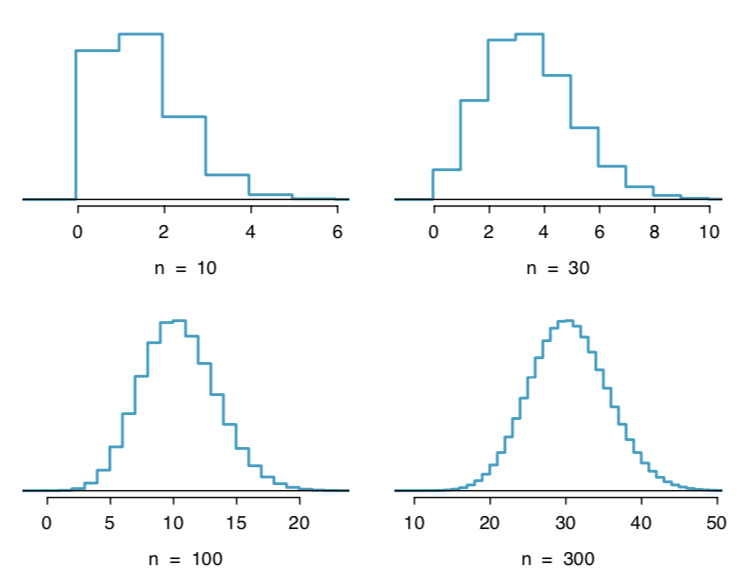
\includegraphics[scale=0.3]{images/nrmbin.png}
    \end{center}
    Each histogram shows a binomial distribution with $p=0.1$.
\end{frame}

\begin{frame}{Example}
    Can we use the normal approximation to estimate the probability of observing 42 or fewer smokers in a sample of 400, if the true proportion of smokers is $p = 0.15$?
\end{frame}

\begin{frame}{Example}
    Can we use the normal approximation to estimate the probability of observing 42 or fewer smokers in a sample of 400, if the true proportion of smokers is $p = 0.15$?
    
    \vspace{12pt}From our previous example, we verified that the binomial model is reasonable. Now,
    \[
        np = 400\times0.15=60
    \]
    and
    \[
        n(1-p) = 400\times 0.85 = 340
    \]
    so both are at least 10 and we may use the normal approximation.
\end{frame}

\begin{frame}{Example}
    For the normal approximation,
    \[
        \mu = np = 400\times0.15 = 60
    \]
    and 
    \[
        \sigma = \sqrt{np(1 − p)} = \sqrt{400\times0.15\times0.85} = 7.14
    \]
\end{frame}

\begin{frame}{Example}
    We want to find the probability of observing 42 or fewer smokers using or $N(\mu=60, \sigma=7.14)$ model. 
    
    \vspace{12pt}We start by finding our Z-score:
    \[
        z = \frac{x-\mu}{\sigma} = \frac{42-60}{7.14} = -2.52
    \]
\end{frame}

\begin{frame}{Example}
    \begin{itemize}
        \item Then, using \texttt{R}, the left-tail area is $0.0059$.
        \item When we calculated this using the binomial distribution, the true probability was $0.0054$.
        \item So this is a pretty good approximation!
    \end{itemize}
\end{frame}

\begin{frame}{Breakdown of the Normal Approximation}
    \begin{itemize}
        \item The normal approximation to the binomial distribution tends to perform poorly when estimating the probability of a small range of counts.
        \item This is true even when $np>10$ and $n(1-p)>10$
    \end{itemize}
\end{frame}

\begin{frame}{Breakdown of the Normal Approximation}
    \begin{itemize}
        \item Suppose we wanted to compute the probability of observing 49, 50, or 51 smokers in 400 when $p = 0.15$.
        \item We know that $np=60>10$ and $n(1-p)=340$, so we might want to apply the normal approximation and use the range 49 to 51.
        \item But this time the approximation and the binomial solution are noticeably different!
        \begin{itemize}
            \item Binomial: 0.0649
            \item Normal: 0.0421
        \end{itemize}
    \end{itemize}
\end{frame}

\begin{frame}{Why Does This Breakdown Happen?}
    \begin{center}
        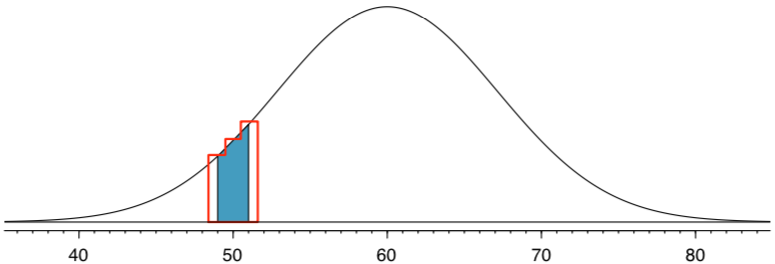
\includegraphics[scale=0.4]{images/approxbreak.png}
    \end{center}
    The binomial probability is shown outlined in red; the normal probability shaded in blue. 
\end{frame}

\begin{frame}{Can We Fix It? Improving the Normal Approximation for Intervals}
    We can usually improve this estimation by modifying our cutoff values.
    \begin{itemize}
        \item Cutoff values for the left side should be reduced by 0.5.
        \item Cutoff values for the right side should be increased by 0.5.
    \end{itemize}
\end{frame}

\begin{frame}{Example}
    \begin{itemize}
        \item Suppose we wanted to compute the probability of observing 49, 50, or 51 smokers in 400 when $p = 0.15$.
        \item Let's try this again with our modification.
        \item For our normal distribution, we used a $N(60, 7.14)$ model.
        \item Our upper value is 51, adjusted to $51+0.5=51.5$.
        \item Our lower value is 49, adjusted to $49-0.5=48.5$.
    \end{itemize}
\end{frame}

\begin{frame}{Example}
    Then
    \[
    z_1 = \frac{x_1 - \mu}{\sigma} = \frac{51.5-60}{7.14} = -1.190476
    \]
    and 
    \[
    z_2 = \frac{x_2 - \mu}{\sigma} = \frac{48.5-60}{7.14} = -1.610644
    \]
\end{frame}

\begin{frame}{Example}
    Now, using \texttt{R}, 
    \begin{align*}
        P(z_2 < Z < z_1) &= P(Z<z_1)-P(Z<z_2) \\
        &= 0.1169297 - 0.05362867 \\
        &= 0.0633
    \end{align*}
\end{frame}

\begin{frame}{Example}
    \begin{center}
        \begin{tabular}{|c|c|c|}
            \hline
            \multicolumn{3}{|c|}{$P(49 \le X \le 51)$} \\ \hline
            \multirow{2}{*}{Binomial} & Normal Approx  & Normal Approx  \\
            & (Adjusted) & (Unadjusted) \\ \hline
            0.0649 & 0.0633 & 0.0421 \\ \hline
        \end{tabular}
    \end{center}
    Making those small adjustments makes a significant difference!
\end{frame}